\documentclass[12pt,169]{beamer}

\usepackage{pablo-beamer}
\date{2015}
\title{Coordonnées de vecteurs}

\begin{document}


\section{Somme de vecteurs}
\begin{frame}
  \begin{center}
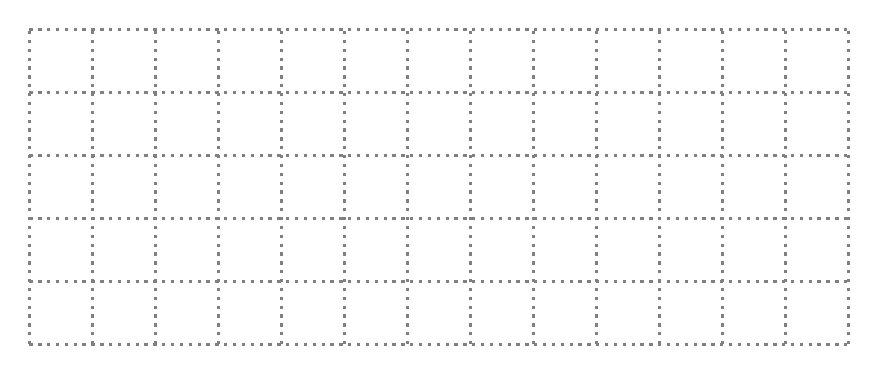
\begin{tikzpicture}[scale=0.8,very thick]
  \draw[dotted,color=gray,step=1] (0,0) grid (13,5);
\end{tikzpicture}
\end{center}

\begin{enumerate}
  \item Tracer un représentant des vecteurs $\vecteur{u}\left( 1,2 \right)$, $\vecteur{v}\left(3;-1 \right)$ et $\vecteur{w}\left( -2;-2 \right)$.
  \item Tracer un représentant des vecteurs $\vecteur{u}+\vecteur{v}$ et $\vecteur{u}+\vecteur{w}$.
  \item Conjecturer un lien entre les coordonnées des vecteurs $\vecteur{u}$, $\vecteur{v}$ et $\vecteur{u}+\vecteur{v}$.
  \item Calculer les coordonnées du vecteur $\vecteur{v}+\vecteur{w}$.
  \item Tracer son représentant, et vérifier le calcul précédent.
\end{enumerate}
\end{frame}

\section{Multiplication de vecteurs par un réel}
\begin{frame}
  \begin{center}
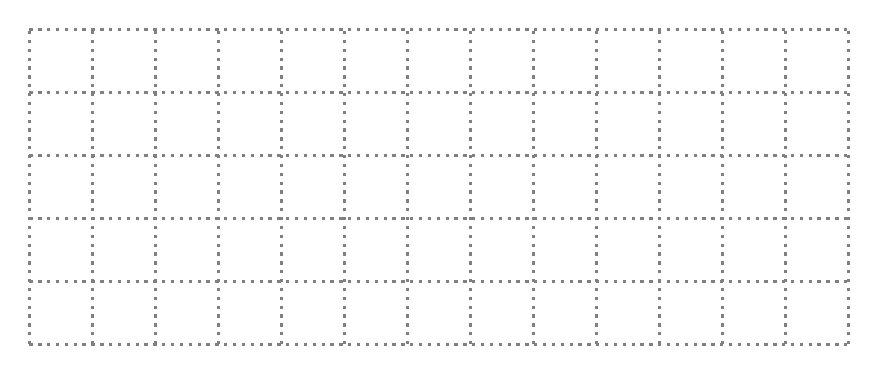
\begin{tikzpicture}[scale=0.8,very thick]
  \draw[dotted,color=gray,step=1] (0,0) grid (13,5);
\end{tikzpicture}
\end{center}

\begin{enumerate}
  \item Tracer un représentant des vecteurs $\vecteur{u}\left( 1,2 \right)$, $\vecteur{v}\left(3;-1 \right)$ et $\vecteur{w}\left( -2;-2 \right)$.
  \item Tracer un représentant des vecteurs $-\vecteur{u}$, $2\vecteur{v}$ et $\frac{1}{2}\vecteur{w}$.
  \item Conjecturer un lien entre les coordonnées des vecteurs $\vecteur{u}$, $\vecteur{v}$ et $\vecteur{u}+\vecteur{v}$.
  \item Quelles sont les coordonnées du vecteur $3\vecteur{u}$ ? Tracer un de ses représentants et vérifier votre réponse.
\end{enumerate}
\end{frame}

\section{Points et Vecteurs}
\begin{frame}
  \begin{center}
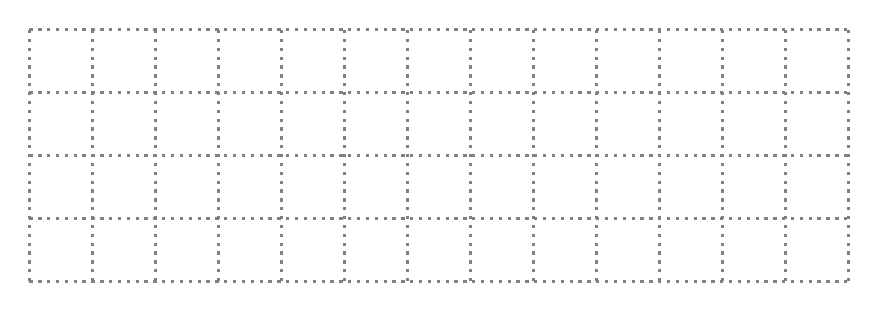
\begin{tikzpicture}[scale=0.8,very thick]
  \draw[dotted,color=gray,step=1] (0,0) grid (13,4);
\end{tikzpicture}
\end{center}

L'objet de l'exercice est de déterminer un lien entre les coordonnées de $A$, $B$ et $\vecteur{AB}$.

Soient $A\left( 2;1 \right)$ et $B\left( -1;1 \right)$ deux points, dans un repère $\left( O, I, J \right)$.
\begin{enumerate}
  \item Avec la relation de Chasles, décomposer le vecteur $\vecteur{AB}$ en passant par le point $O$.
  \item Traduire cette égalité de vecteurs par une égalité de coordonnées.
  \item Lire graphiquement les coordonnées de $\vecteur{AB}$, et vérifier votre réponse à la question précédente.
\end{enumerate}
\end{frame}

\end{document}
